\documentclass[tikz,border=12pt]{standalone}
\usepackage[T1]{fontenc}
\usepackage{lmodern}
\usetikzlibrary{positioning,arrows.meta,shapes.geometric}

\begin{document}
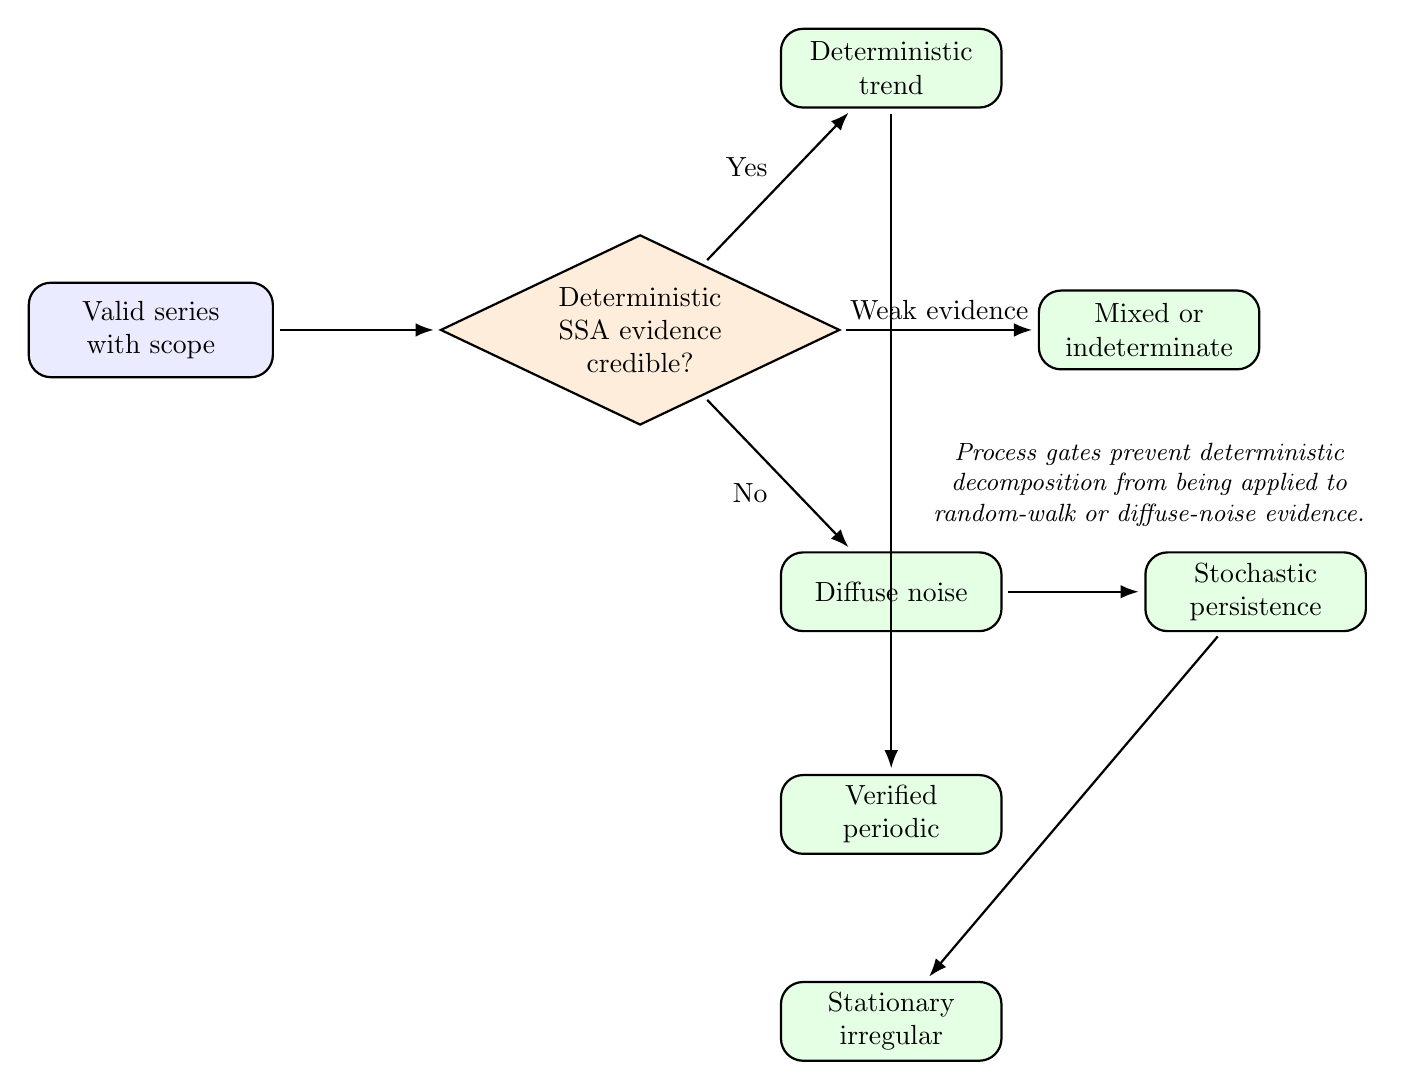
\begin{tikzpicture}[
  box/.style={draw, rounded corners=8pt, align=center, minimum width=3.1cm, minimum height=1.2cm, fill=blue!8, line width=0.8pt},
  decision/.style={draw, diamond, align=center, aspect=2.1, fill=orange!14, line width=0.8pt},
  outcome/.style={draw, rounded corners=8pt, align=center, minimum width=2.8cm, minimum height=1.0cm, fill=green!10, line width=0.8pt},
  note/.style={font=\small\itshape, align=center},
  arrow/.style={-Latex, thick, shorten >=2pt, shorten <=2pt}
]

\node[box] (data) {Valid series\\with scope};
\node[decision, right=2.1cm of data] (suitable) {Deterministic\\SSA evidence\\credible?};
\node[outcome, above right=2.2cm and 0.5cm of suitable] (trend) {Deterministic\\trend};
\node[outcome, below right=2.2cm and 0.5cm of suitable] (noise) {Diffuse noise};
\node[outcome, right=2.5cm of suitable] (mixed) {Mixed or\\indeterminate};
\node[outcome, right=1.8cm of noise] (persist) {Stochastic\\persistence};
\node[outcome, below=1.8cm of noise] (periodic) {Verified\\periodic};
\node[outcome, below=1.6cm of periodic] (stationary) {Stationary\\irregular};

\draw[arrow] (data) -- (suitable);
\draw[arrow] (suitable) -- node[above left]{Yes} (trend);
\draw[arrow] (suitable) -- node[below left]{No} (noise);
\draw[arrow] (suitable) -- node[above]{Weak evidence} (mixed);
\draw[arrow] (trend) -- (periodic);
\draw[arrow] (noise) -- (persist);
\draw[arrow] (persist) -- (stationary);

\node[note, below=0.8cm of mixed, text width=5.6cm] {Process gates prevent deterministic decomposition from being applied to random-walk or diffuse-noise evidence.};

\end{tikzpicture}
\end{document}
